\documentclass[12pt,notitlepage]{article}
\usepackage[utf8]{inputenc}
\usepackage{natbib}
\usepackage[dutch]{babel}
\usepackage{graphicx}
\usepackage{colortbl}
\usepackage{blindtext}
\usepackage[final]{pdfpages}
\usepackage[a4paper, total={6.3in,9in},footskip=76pt]{geometry}


% make section start with Alphabet letters
\renewcommand{\thesection}{\alph{section}}

% plots
\usepackage{pgfplots}
\pgfplotsset{compat=1.8}
\pgfplotsset{mystyle/.style={%
        width=6in,
        ylabel={Aantal Swaps},
        xlabel={Aantal studenten},
        xmin=0,xmax=160000,
        scaled y ticks = false,
        scaled x ticks = false,	
       	x tick label style={rotate=45, anchor=north east, inner sep=0mm},
       	legend pos=north west
        }}


\usepackage{titlesec}
\titlespacing\section{0pt}{12pt plus 4pt minus 2pt}{0pt plus 2pt minus 2pt}
\titlespacing\subsection{0pt}{0pt plus 4pt minus 2pt}{0pt plus 2pt minus 2pt}
\titlespacing\subsubsection{0pt}{12pt plus 4pt minus 2pt}{0pt plus 2pt minus 2pt}

% turn off word breaking
\usepackage{hyphenat}
\hyphenpenalty 10000
\exhyphenpenalty 10000
\raggedright

% make paragraphs with line spacing
\setlength{\parskip}{\baselineskip}%
\setlength{\parindent}{0pt}%


% Set up code listings for Java
\usepackage{listings}
\usepackage{color}

\definecolor{dkgreen}{rgb}{0,0.6,0}
\definecolor{gray}{rgb}{0.5,0.5,0.5}
\definecolor{mauve}{rgb}{0.58,0,0.82}

\lstset{frame=tb,
  language=Java,
  aboveskip=3mm,
  belowskip=3mm,
  showstringspaces=false,
  columns=flexible,
  basicstyle={\small\ttfamily},
  numbers=none,
  numberstyle=\tiny\color{gray},
  keywordstyle=\color{blue},
  commentstyle=\color{dkgreen},
  stringstyle=\color{mauve},
  breaklines=true,
  breakatwhitespace=true,
  tabsize=3
}

\begin{document}


%----------------------------------------------------------------------------------------
%	ONDERZOEKSVOORSTEL
%----------------------------------------------------------------------------------------

\begin{titlepage}

\newcommand{\HRule}{\rule{\linewidth}{0.5mm}}

\center % Center everything on the page

%----------------------------------------------------------------------------------------
%	HEADING SECTIONS
%----------------------------------------------------------------------------------------
\begin{figure}[h!]
\centering

\includegraphics[scale=0.5]{hva-logo.png}
\end{figure}
\textsc{\LARGE Hogeschool van Amsterdam}\\[1.5cm] % Name of your university/college
\textsc{\Large Sorting \& Searching}\\[0.5cm] % Major heading such as course name
\textsc{\large Efficiëntie van geavanceerde sorteeralgoritmes}\\[0.5cm] % Minor heading such as course title

%----------------------------------------------------------------------------------------
%	TITLE SECTION
%----------------------------------------------------------------------------------------

\HRule \\[0.4cm]
{ \huge \bfseries Practicum 1}\\[0.2cm] % Title of your document
\HRule \\[1.2cm]

% Optimalisatie van gegevensverwerking voor iLocate

%----------------------------------------------------------------------------------------
%	AUTHOR SECTION
%----------------------------------------------------------------------------------------

\begin{minipage}{0.4\textwidth}
\begin{flushleft} \large
\emph{Author:}\\
Robert \textsc{Bakker} % Your name
\linebreak
\linebreak
\emph{Studentnummer:}\\
500689284
\linebreak
\linebreak
\emph{Klas:}\\
IVSE4

\end{flushleft}
\end{minipage}
~
\begin{minipage}{0.4\textwidth}
\begin{flushright} \large
\emph{Author:}\\
Mark \textsc{van der Steenhoven} % Your name
\linebreak
\linebreak
\emph{Studentnummer:}\\
500693745
\linebreak
\linebreak
\emph{Klas:}\\
IVSE4
\end{flushright}
\end{minipage}\\[4cm]

%----------------------------------------------------------------------------------------
%	DATE SECTION
%----------------------------------------------------------------------------------------

{\large Blok 2, 2016 - 2017}\\[3cm] % Date, change the \today to a set date if you want to be precise

%----------------------------------------------------------------------------------------
%	LOGO SECTION
%----------------------------------------------------------------------------------------

%\includegraphics{Logo}\\[1cm] % Include a department/university logo - this will require the graphicx package

%----------------------------------------------------------------------------------------

\vfill % Fill the rest of the page with whitespace

\end{titlepage}


%----------------------------------------------------------------------------------------
%	TABLE OF CONTENTS
%----------------------------------------------------------------------------------------
\renewcommand{\contentsname}{Inhoudsopgave}
\tableofcontents
\clearpage

%----------------------------------------------------------------------------------------
%	Opdracht a
%----------------------------------------------------------------------------------------

\section{Resultaten van studenten sorteren met een advanced sort}
Voor deze opdracht wordt gebruik gemaakt van de volgende Student-klasse:

\begin{lstlisting}
public class Student implements Comparable<Student> {

    private String group;
    private int studentNumber;
    private float grade;

    public Student(String group, int studentNumber, float grade) {
        this.group = group;
        this.studentNumber = studentNumber;
        this.grade = grade;
    }
    
    // Getters and Setters
    
    @Override
    public int compareTo(Student that) {
        if (this.grade < that.getGrade()) return -1;
        if (this.grade > that.getGrade()) return 1;
        if(this.studentNumber < that.getStudentNumber()) return -1;
        if(this.studentNumber > that.getStudentNumber()) return 1;

        return 0;
    }
}
\end{lstlisting}

Waarbij het met name gaat om de implementatie van de Comparable-interface. Als twee Student-objecten met elkaar worden vergeleken, wordt in eerste instantie gekeken naar het cijfer (grade). Mochten de cijfers niet groter of kleiner zijn dan elkaar oftwel gelijk zijn, wordt er teruggevallen op een vergelijking op het studentnummer.

\clearpage
\subsection{Quicksort implemenatie}
Hieronder de Quicksort implementatie voor de experimenten in paragraaf a.2 met zoveel mogelijk uitleg in het codecommentaar:
\begin{lstlisting}
    // De quicksort accepteert een lijst van objecten met een Comparable
    // interface (bijv. de Student-klasse), het beginpunt vanaf links,
    // en het beginpunt vanaf rechts 
    private void quicksort(Comparable[] list, int low, int high) {
        // Neem het middelpunt van de array als spil (draaipunt)
        Comparable pivot = list[low + (high - low) / 2];
        int i = low; // linkerkant
        int j = high; // rechterkant
        // Partitioneren
        while (i <= j) {
            // Wanneer object vanaf links kleiner is dan de spil
            // Verschuif naar de volgende in de linkerlijst
            while (list[i].compareTo(pivot) < 0) {
                i++;
            }
            // Wanneer object vanaf rechts groter is dan de spil
            // Verschuif naar de volgende in de rechterlijst
            while (list[j].compareTo(pivot) > 0) {
                j--;
            }
            // Als er een index van de linkerlijst is gevonden, met een waarde
            // die groter is dan de spil, en een index in de rechterlijst met
            // een waarde die kleiner is dan de spil, moeten de 2 waarden
            // worden omgedraaid
            if (i <= j) {
                swap(list, i, j);
                i++; j--;
            }
        }
        // Hetzelfde voor de rest van de linkerlijst
        if (low < j) quicksort(list, low, j);
        // en voor de rechterlijst
        if (high > i) quicksort(list, i, high);
    }
    private void swap(Comparable[] list, int i, int j) {
        Comparable temp = list[i];
        list[i] = list[j];
        list[j] = temp;
        swaps++; // Tel het aantal swaps
    }
\end{lstlisting}
\clearpage
Om te laten zien dat het werkt, de output van de cijfers voor het en het sorten met een lijst van 15 elementen:

\begin{figure}[h!]
\centering
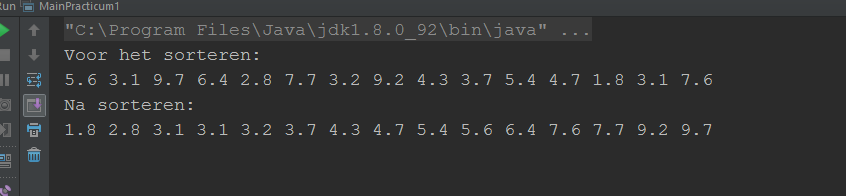
\includegraphics[scale=0.8]{quicksort_test.png}
\end{figure}

\subsection{Resultaten experiment}
Het experiment bestond uit het meten van de tijd die de Quicksort implementatie in de vorige paragraaf nodig heeft om lijsten met verschillende aantallen studenten te sorteren.

\begin{lstlisting}
int[] numberOfStudents = {10000, 20000, 40000, 80000, 160000};
// N_EXPERIMENTS = 5
// Houd alle resultaten bij in een 2-dimensionale array.
// Hier mee kunnen we uiteindelijk het gemiddelde berekenen van ieder experiment
long[][] quicksortResults = new long[numberOfStudents.length][N_EXPERIMENTS];

for (int i = 0; i < numberOfStudents.length; i++) {
    for (int j = 0; j < N_EXPERIMENTS; j++) {
        ResultList list = StudentListGenerator.generate(numberOfStudents[i]);
        list.shuffle(); // StdRandom.shuffle()
        list.quicksort(); // De Quicksort implementatie
        quicksortResults[i][j] = list.getSwaps();
    }
}
\end{lstlisting}

Het experiment is meerdere keren uitgevoerd en daarvan is het gemiddelde genomen. Dit zijn de resultaten:
Meetresultaten: 


\subsubsection{Aantal swaps}
\begin{center}
	\begin{tabular}{|>{\columncolor[RGB]{230, 242, 255}}l|l|l|l|l|l|l|}
	\hline
	Aantal studenten ($n$) & Run 1 & Run 2 & Run 3 & Run 4 & Run 5 & Gemiddeld ($t$) \\
	\hline
	10000 & 33583 & 33790 & 33239 & 33678 & 33255 & 33509 \\
	\hline
	20000 & 72213 & 71764 & 71754 & 71722 & 71561 & 71802 \\
	\hline
	40000 & 152818 & 152305 & 152601 & 153322 & 151588 & 152526 \\
	\hline
	80000 & 323338 & 321402 & 325179 & 325067 & 323066 & 323610 \\
	\hline
	160000 & 686829 & 678957 & 687429 & 680257 & 683060 & 683306 \\
	\hline
	\end{tabular}
\end{center}

\subsubsection{Aantal compares}
\begin{center}
	\begin{tabular}{|>{\columncolor[RGB]{230, 242, 255}}l|l|l|l|l|l|l|}
	\hline
	Aantal studenten (n) & Run 1 & Run 2 & Run 3 & Run 4 & Run 5 & Gemiddeld (t) \\
	\hline
	10000 & 118702 & 103213 & 110760 & 106625 & 96812 & 107222 \\
	\hline
	20000 & 233464 & 227495 & 253906 & 242096 & 241585 & 239709 \\
	\hline
	40000 & 525474 & 547440 & 506842 & 487517 & 553209 & 524096 \\
	\hline
	80000 & 1126047 & 1071245 & 1088298 & 1252791 & 1054870 & 1118650 \\
	\hline
	160000 & 2327269 & 2399714 & 2616240 & 2263507 & 2298539 & 2381053 \\
	\hline
	\end{tabular}
\end{center}

%De tijd die we gemeten hebben om 10.000 studenten te sorteren ligt is gemiddeld \textsf{51 ms}.
%Hierbij hebben Java met de VM optie \textsf{-Djava.compiler=NONE} uitgevoerd om optimalisaties uit te schakelen. Die optie voorkomt dat Java het programma met extra optimalisaties gaat uitvoeren.


\subsection{Efficiëntie}

Door de meetresultaten naast verschillende Big O notaties te houden kunnen we bepalen welke Big O notatie erbij hoort.
\begin{center}
	\begin{tabular}{|>{\columncolor[RGB]{230, 242, 255}}l|l||l|l||l||l|l|}
 \hline
 \multicolumn{2}{|c||}{Meetresultaten} & \multicolumn{2}{c||}{$O(n^m)$} & \multicolumn{1}{c||}{$O(log\ n)$} & \multicolumn{2}{|>{\columncolor[RGB]{117, 200, 32}}c|}{$O(n\ log\ n)$} \\
 \hline	
	\hline
	$n$ & $t$ & Factor ($f$) & $m = log(f, 2)$ & Verschil & $t / log\ n$ & Factor ($f$) \\
	\hline
	10000 & 33509 & - & - & - & 3638.19 & - \\
	\hline
	20000 & 71802 & 2.14 & 1.10 & 38293 & 7250.17 & 1.99 \\
	\hline
	40000 & 152526 & 2.12 & 1.09 & 80724 & 14393.82 & 1.99 \\
	\hline
	80000 & 323610 & 2.12 & 1.09 & 171084 & 28663.97 & 1.99 \\
	\hline
	160000 & 683306 & 2.11 & 1.08 & 359696 & 57023.29 & 1.99 \\
	\hline
	\end{tabular}
\end{center}

Uit de tabel blijkt dat $O(n\ log\ n)$ een constante heeft en de factor kom het dichtst bij een verdubbeling uit. Bij de andere Big O's zien we dat de waardes niet constant zijn. Het is geen O(n) want de factor verschilt per verdubbeling van het aantal studenten. Ook geen $O(log\ n)$ want de toename is niet constant. De goede is groen gemarkeerd en is dus $O(n\ log\ n)$.

%\begin{tikzpicture}
%  \begin{axis}[mystyle]
%\addlegendentry{$Big O$}
%\addplot+[smooth] coordinates
%{(10000, 33509) (20000, 71802) (40000, 152526) (80000, 323610) (160000, 683306) };
%  \end{axis}
%\end{tikzpicture}

% \begin{center}
% 	\begin{tabular}{|l|l|l|l|l|l|l|}
% 	\hline
% 	n & t & Vergrotingsfactor (f) & log (f, 2) & (t + 1) - t & t / log n & Vergrotingsfactor (f) \\
% 	\hline
% 	10000 & 107222 & - & - & - & 11641.48 & - \\
% 	\hline
% 	20000 & 239709 & 2.24 & 1.16 & 132487 & 24204.50 & 2.08 \\
% 	\hline
% 	40000 & 524096 & 2.19 & 1.13 & 284387 & 49458.72 & 2.04 \\
% 	\hline
% 	80000 & 1118650 & 2.13 & 1.09 & 594554 & 99085.17 & 2.00 \\
% 	\hline
% 	160000 & 2381053 & 2.13 & 1.09 & 1262403 & 198703.75 & 2.01 \\
% 	\hline
% 	\end{tabular}
% \end{center}

\clearpage
%----------------------------------------------------------------------------------------
%	Opdracht b
%----------------------------------------------------------------------------------------
\section{Verbetering toevoegen aan algoritme}

\subsection{Median-of-Three implementatie}

We nemen dezelfde code als van Quicksort als uitgangspunt.
De implementatie van het partitioneren blijft hetzelfde, we veranderen de manier waarop de spil wordt berekend, door middel van een steekproef ter grootte van 3 en daarbij het middelste resultaat te nemen. Dit zou het partitioneren efficienter moeten maken, maar het berekenen van de spil wordt minder efficient.

\begin{lstlisting}

   int i = low, j = high;
   int n = high - low + 1;
   int mid = low + n / 2;

   // Bepaal de spil nu door middel van een steekproefgrootte van 3 en
   // pak daarvan de index van middelste waarde
    int m = median3(list, low, mid, high);
    Comparable pivot = list[m];
    swap(list, m, low);

\end{lstlisting}

Hierbij gebruiken we een nieuwe median3() methode die de index van de waarde bepaald die in het midden van de steekproef ligt:

\begin{lstlisting}
private int median3(Comparable[] list, int a, int b, int c) {
    if (list[a].compareTo(list[b]) <= 0) {
        if (list[b].compareTo(list[c]) <= 0)
            return b; // a <= b <= c, dus b ligt in het midden
        else if (list[a].compareTo(list[c]) <= 0)
            return c; // a <= c < b, dus c ligt in het midden
        else
            return a; // c < a < b, dus a ligt in het midden
    } else {
        if (list[a].compareTo(list[c]) <= 0)
            return a; // b < a <= c, dus a ligt in het midden
        else if (list[b].compareTo(list[c]) <= 0)
            return c; // b <= c < a, dus c ligt in het midden
        else
            return b; // c < b < a, dus b ligt in het midden
    }
}
\end{lstlisting}

Om te laten zien dat het werkt, de output van de cijfers voor het en het sorten met een lijst van 15 elementen:

\begin{figure}[h!]
\centering
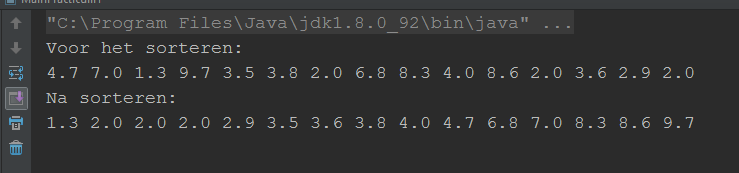
\includegraphics[scale=0.8]{median3_test.png}
\end{figure}


\subsection{Resultaten experiment}

Hetzelfde als het vorige experiment, maar wordt de spil op een andere manier bepaald, via de Median-of-Three methode.

\subsubsection{Aantal swaps}

\begin{center}
	\begin{tabular}{|>{\columncolor[RGB]{230, 242, 255}}l|l|l|l|l|l|l|}
	\hline
	Aantal studenten (n) & Run 1 & Run 2 & Run 3 & Run 4 & Run 5 & Gemiddeld (t) \\
	\hline
	10000 & 45119 & 44828 & 44879 & 45239 & 44388 & 44890 \\
	\hline
	20000 & 94704 & 94738 & 94758 & 94865 & 94472 & 94707 \\
	\hline
	40000 & 199194 & 196615 & 197957 & 199295 & 198320 & 198276 \\
	\hline
	80000 & 412507 & 415379 & 417447 & 416018 & 413535 & 414977 \\
	\hline
	160000 & 859779 & 865425 & 866948 & 861188 & 860469 & 862761 \\
	\hline
	\end{tabular}
\end{center}

\subsubsection{Aantal vergelijkingen}

\begin{center}
	\begin{tabular}{|>{\columncolor[RGB]{230, 242, 255}}l|l|l|l|l|l|l|}
	\hline
	Aantal studenten (n) & Run 1 & Run 2 & Run 3 & Run 4 & Run 5 & Gemiddeld (t) \\
	\hline
	10000 & 96909 & 95691 & 94924 & 103175 & 101154 & 98370 \\
	\hline
	20000 & 212020 & 208320 & 232209 & 217651 & 212189 & 216477 \\
	\hline
	40000 & 474403 & 468668 & 472091 & 456692 & 461716 & 466714 \\
	\hline
	80000 & 1058276 & 1040906 & 954451 & 935949 & 994185 & 996753 \\
	\hline
	160000 & 2046106 & 2031889 & 2369335 & 2236124 & 2223647 & 2181420 \\
	\hline
	\end{tabular}
\end{center}

We zien ten opzichte van de resultaten zonder Median-of-3 dat het aantal swaps hoger is, maar het aantal vergelijkingen minder. Dit wijst dus op een goede verdeling van de twee lijsten. 

\clearpage

\subsection{Efficiëntie}

\begin{center}
	\begin{tabular}{|>{\columncolor[RGB]{230, 242, 255}}l|l||l|l||l||l|l|}
 \hline
 \multicolumn{2}{|c||}{Meetresultaten} & \multicolumn{2}{c||}{$O(n^m)$} & \multicolumn{1}{c||}{$O(log\ n)$} & \multicolumn{2}{|>{\columncolor[RGB]{117, 200, 32}}c|}{$O(n\ log\ n)$} \\
 \hline	
	\hline
	$n$ & $t$ & Factor ($f$) & $m = log(f, 2)$ & Verschil & $t / log\ n$ & Factor ($f$) \\
	\hline
	10000 & 44890 & - & - & - & 4873.87 & - \\
	\hline
	20000 & 94707 & 2.11 & 1.08 & 49817 & 9562.99 & 1.96 \\
	\hline
	40000 & 198276 & 2.09 & 1.07 & 103569 & 18711.22 & 1.96 \\
	\hline
	80000 & 414977 & 2.09 & 1.07 & 216701 & 36756.87 & 1.96 \\
	\hline
	160000 & 862761 & 2.08 & 1.06 & 447784 & 71999.17 & 1.96 \\
	\hline
	\end{tabular}
\end{center}

Ook hier zien we weer dat $O(n\ log\ n)$ een constante heeft en de factor het dichtst bij een verdubbeling zit. Bij de andere Big O's zien we dat de waardes niet constant zijn. Het is geen O(n) want de factor verschilt per verdubbeling van het aantal studenten. Ook geen $O(log\ n)$ want de toename is niet constant. De goede is groen gemarkeerd en is dus $O(n\ log\ n)$.

Wat nog op valt is dat de factor kleiner is ten opzichte dat van de Quicksort zonder Median-of-3.

\clearpage
%----------------------------------------------------------------------------------------
%	Opdracht c
%----------------------------------------------------------------------------------------
\section{Resultaten in een Binary Search Tree en implementatie van rank()}

\subsection{Duplicaten}
Om duplicaten(studenten met hetzelfde cijfer) in de BST te kunnen plaatsen, krijgt de Node binnen de BST in plaats van 1 waarde, een lijst van waardes:

\begin{lstlisting}
private class Node {

    private Key key;
    private List<Value> val = new LinkedList<Value>(); // Lijst i.p.v. alleen Value
    private Node left, right;
    private int N;

    public Node(Key key, Value val, int N) {
        this.key = key;
        this.val.add(val); // Voeg toe aan lijst
        this.N = N;
    }
}
\end{lstlisting}

Het probleem met de implementatie uit het boek is dat wanneer, via de put() methode, er 2 Nodes worden toegevoegd met dezelfde Key, de Value wordt overschreven. Dit is opgelost door het aan de List toe te voegen:

\begin{lstlisting}
private Node put(Node x, Key key, Value val) {
    if (x == null) {
        return new Node(key, val, 1);
    }
    int cmp = key.compareTo(x.key);
    if (cmp < 0) {
        x.left = put(x.left, key, val);
    } else if (cmp > 0) {
        x.right = put(x.right, key, val);
    } else {
        // Voeg toe aan lijst i.p.v. overschrijven single value
        x.val.add(val); 
    }
    x.N = size(x.left) + size(x.right) + 1;
    return x;
}
\end{lstlisting}
\clearpage
En de get() method geeft nu in plaats van 1 waarde, een lijst terug:

\begin{lstlisting}
private List<Value> get(Node x, Key key) {
    if (x == null) {
        return null;
    }
    int cmp = key.compareTo(x.key);
    if (cmp < 0) {
        return get(x.left, key);
    } else if (cmp < 0) {
        return get(x.right, key);
    } else {
        return x.val;
    }
}
\end{lstlisting}

\subsection{Rank()}
\subsubsection{BST implementatie rank()}

\begin{lstlisting}

 private int rank(Key key, Node x) {
        if (x == null) {
            return 0;
        }
        int cmp = key.compareTo(x.key);
        if (cmp < 0) {
            return rank(key, x.left);
        } else if (cmp > 0) {
            return x.val.size() + size(x.left) + rank(key, x.right);
        } else {
            return size(x.left);
        }
    }
\end{lstlisting}

\clearpage
\subsubsection{Voorbeeld data voor rank}

De input is een lijst van studenten bestaande uit een cijfer en studentnummer. De input set bestaat uit 16 studenten en de cijfers aan de hand van het voorbeeld in de opdrachtomschrijving. Op deze list voeren wij de rank method uit om een overzicht te krijgen hoeveel studenten lager dan een bepaald cijfer hebben behaald.
\linebreak
\begin{lstlisting}
float[] testGrades = {10f, 9f, 9f, 8f, 8f, 8f,
 7f, 7f, 6f, 6f, 6f, 6f, 6f, 5f, 3f, 2f};

// Maak een lijstje van studenten aan
Student[] studentList = 
	StudentListGenerator.generate(testGrades.length).getList();

// Geef de studenten de test waardes als cijfer
for (int i = 0; i < testGrades.length; i++) {
    studentList[i].setGrade(testGrades[i]);
}
BST<Float, Integer> bst = new BST<>();
// Shuffle met als doel de BST gebalanceerder te maken
StdRandom.shuffle(studentList); 
for (Student s : studentList) {
    bst.put(s.getGrade(), s.getStudentNumber());
}

// Rank elk cijfer
for (int i = 1; i <= 10; i++) {
    System.out.println("Grade: " + i + ", rank: " + bst.rank((float) i));
}
\end{lstlisting}

\textbf{Output}

Grade: 1, rank: 0\\
Grade: 2, rank: 0\\
Grade: 3, rank: 1\\
Grade: 4, rank: 2\\
Grade: 5, rank: 2\\
Grade: 6, rank: 3\\
Grade: 7, rank: 8\\
Grade: 8, rank: 10\\
Grade: 9, rank: 13\\
Grade: 10, rank: 15\\

\end{document}

\end{document}